%%%%%%%%%%%%%%%%%%%%%%%%%%%%%%%%%%%%%%%%%
% Arsclassica Article
% LaTeX Template
% Version 1.1 (1/8/17)
%
% This template has been downloaded from:
% http://www.LaTeXTemplates.com
%
% Original author:
% Lorenzo Pantieri (http://www.lorenzopantieri.net) with extensive modifications by:
% Vel (vel@latextemplates.com)
%
% License:
% CC BY-NC-SA 3.0 (http://creativecommons.org/licenses/by-nc-sa/3.0/)
%
%%%%%%%%%%%%%%%%%%%%%%%%%%%%%%%%%%%%%%%%%

%----------------------------------------------------------------------------------------
%	PACKAGES AND OTHER DOCUMENT CONFIGURATIONS
%----------------------------------------------------------------------------------------

\documentclass[
10pt, % Main document font size
a4paper, % Paper type, use 'letterpaper' for US Letter paper
oneside, % One page layout (no page indentation)
%twoside, % Two page layout (page indentation for binding and different headers)
headinclude,footinclude, % Extra spacing for the header and footer
BCOR5mm, % Binding correction
]{scrartcl}

%%%%%%%%%%%%%%%%%%%%%%%%%%%%%%%%%%%%%%%%%
% Arsclassica Article
% Structure Specification File
%
% This file has been downloaded from:
% http://www.LaTeXTemplates.com
%
% Original author:
% Lorenzo Pantieri (http://www.lorenzopantieri.net) with extensive modifications by:
% Vel (vel@latextemplates.com)
%
% License:
% CC BY-NC-SA 3.0 (http://creativecommons.org/licenses/by-nc-sa/3.0/)
%
%%%%%%%%%%%%%%%%%%%%%%%%%%%%%%%%%%%%%%%%%

%----------------------------------------------------------------------------------------
%	REQUIRED PACKAGES
%----------------------------------------------------------------------------------------

\usepackage[
nochapters, % Turn off chapters since this is an article        
beramono, % Use the Bera Mono font for monospaced text (\texttt)
eulermath,% Use the Euler font for mathematics
pdfspacing, % Makes use of pdftex’ letter spacing capabilities via the microtype package
dottedtoc % Dotted lines leading to the page numbers in the table of contents
]{classicthesis} % The layout is based on the Classic Thesis style

\usepackage{arsclassica} % Modifies the Classic Thesis package

\usepackage[T1]{fontenc} % Use 8-bit encoding that has 256 glyphs

\usepackage[utf8]{inputenc} % Required for including letters with accents

\usepackage{graphicx} % Required for including images
\graphicspath{{Figures/}} % Set the default folder for images

\usepackage{enumitem} % Required for manipulating the whitespace between and within lists

\usepackage{lipsum} % Used for inserting dummy 'Lorem ipsum' text into the template

\usepackage{subfig} % Required for creating figures with multiple parts (subfigures)

\usepackage{amsmath,amssymb,amsthm} % For including math equations, theorems, symbols, etc

\usepackage{varioref} % More descriptive referencing


%----------------------------------------------------------------------------------------
%	THEOREM STYLES
%---------------------------------------------------------------------------------------

\theoremstyle{definition} % Define theorem styles here based on the definition style (used for definitions and examples)
\newtheorem{definition}{Definition}

\theoremstyle{plain} % Define theorem styles here based on the plain style (used for theorems, lemmas, propositions)
\newtheorem{theorem}{Theorem}

\theoremstyle{remark} % Define theorem styles here based on the remark style (used for remarks and notes)

%----------------------------------------------------------------------------------------
%	HYPERLINKS
%---------------------------------------------------------------------------------------

\hypersetup{
%draft, % Uncomment to remove all links (useful for printing in black and white)
colorlinks=true, breaklinks=true, bookmarks=true,bookmarksnumbered,
urlcolor=webbrown, linkcolor=RoyalBlue, citecolor=webgreen, % Link colors
pdftitle={}, % PDF title
pdfauthor={\textcopyright}, % PDF Author
pdfsubject={}, % PDF Subject
pdfkeywords={}, % PDF Keywords
pdfcreator={pdfLaTeX}, % PDF Creator
pdfproducer={LaTeX with hyperref and ClassicThesis} % PDF producer
} % Include the structure.tex file which specified the document structure and layout

\hyphenation{Fortran hy-phen-ation} % Specify custom hyphenation points in words with dashes where you would like hyphenation to occur, or alternatively, don't put any dashes in a word to stop hyphenation altogether

%----------------------------------------------------------------------------------------
%	TITLE AND AUTHOR(S)
%----------------------------------------------------------------------------------------

\title{\normalfont\spacedallcaps{Elementary particle}} % The article title

%\subtitle{Subtitle} % Uncomment to display a subtitle

\author{\spacedlowsmallcaps{Chenxi Gu*}} % The article author(s) - author affiliations need to be specified in the AUTHOR AFFILIATIONS block

\date{} % An optional date to appear under the author(s)

%----------------------------------------------------------------------------------------

\begin{document}

%----------------------------------------------------------------------------------------
%	HEADERS
%----------------------------------------------------------------------------------------

\renewcommand{\sectionmark}[1]{\markright{\spacedlowsmallcaps{#1}}} % The header for all pages (oneside) or for even pages (twoside)
%\renewcommand{\subsectionmark}[1]{\markright{\thesubsection~#1}} % Uncomment when using the twoside option - this modifies the header on odd pages
\lehead{\mbox{\llap{\small\thepage\kern1em\color{halfgray} \vline}\color{halfgray}\hspace{0.5em}\rightmark\hfil}} % The header style

\pagestyle{scrheadings} % Enable the headers specified in this block

%----------------------------------------------------------------------------------------
%	TABLE OF CONTENTS & LISTS OF FIGURES AND TABLES
%----------------------------------------------------------------------------------------

\maketitle % Print the title/author/date block

\setcounter{tocdepth}{2} % Set the depth of the table of contents to show sections and subsections only

\tableofcontents % Print the table of contents

\listoffigures % Print the list of figures

\listoftables % Print the list of tables

%----------------------------------------------------------------------------------------
%	ABSTRACT
%----------------------------------------------------------------------------------------

\section*{Abstract} % This section will not appear in the table of contents due to the star (\section*)

In this paper we review some elementary particle.They are very important part of standard model.Such as $\pi$,$K$.Mass, Width, Angular momentum, Parity, Isospin are our point.They may interact through the strong electromagnetic weak or through some unknown force.The purpose of this review is to provide a guide for future searches what is known, what is not known. This is very necessary for the beginner.


%----------------------------------------------------------------------------------------
%	AUTHOR AFFILIATIONS
%----------------------------------------------------------------------------------------

\let\thefootnote\relax\footnotetext{* \textit{ Department of engineering physics, Tsinghua University, Pekin, China}}



%----------------------------------------------------------------------------------------

%\newpage % Start the article content on the second page, remove this if you have a longer abstract that goes onto the second page

%----------------------------------------------------------------------------------------
%	INTRODUCTION
%----------------------------------------------------------------------------------------



 
%----------------------------------------------------------------------------------------
%	PARTICLE TREE
%----------------------------------------------------------------------------------------

\section{Particle Tree}
There are so many elementary particles, So the best way is classify them.All elementary particles are made up quarks.In this paper we just focus on the meson and baryon which composed of 2 or 3 quarks.

\begin{enumerate}[noitemsep] % [noitemsep] removes whitespace between the items for a compact look
\item Light Unflavored Mesons
\item Strange Mesons
\item N Baryons
\item $\Delta$ Baryons
\item $\Lambda$ Baryons
\item $\Sigma$ Baryons
\item $\Xi$ Baryons
\end{enumerate}

%------------------------------------------------

\subsection{Light Unflavored Mesons}
What is light unflavored mesons? In the quantum mechanic, we can use some quantum numbers to describe a quantum system.For the elementary particles, we usually use $S$, $C$ and $B$. Light unflavored mesons is $S=C=B=0$.

\begin{table}[hbt]
\caption{Light Unflavored Mesons}
\centering
\begin{tabular}{lllr}
\toprule
Particle & Mass(MeV) & Width & $I^G(J^{PC})$ \\
\midrule
$\pi^{\pm}$ & $139.57018\pm0.00035$ & $(2.6033\pm0.0005)*10^{-8}s$& $1^-(0^-)$ \\
$\pi^0$ & $134.9766\pm0.0006$ &$(8.52\pm0.18)*10^{-17}s$ & $1^-(0^{-+})$ \\
$\eta$ & $547.862\pm0.017$ & $1.31\pm0.05keV$ &$0^+(0^{-+})$\\
$\eta^{'}$ & $957.78\pm0.06$ & $0.197\pm0.009MeV$ &$0^+(0^{-+})$ \\
$\rho$ &$775.26\pm0. 25$ & $149.1\pm0.8MeV$&$1^+(1^{--})$ \\
$\omega$ & $782.65\pm0.12$ & $8.49\pm0.08MeV$ &$0^-(1^{--})$ \\
$\phi$ & $1019.461\pm0.019$ & $4.266\pm0.031MeV$ &$0^-(1^{--})$ \\
\bottomrule
\end{tabular}
\label{tab:label}
\end{table}
Some particles are not the C eigenstate, such as $\pi^{\pm}$. We also could use lifetime to express the width, because we have $\Gamma=\frac{\hbar}{\tau}$.


\subsection{Strange Mesons}
Strange mesons are $C=B=0, S=\pm1$.
\begin{table}[hbt]
\caption{Strange Mesons}
\centering
\begin{tabular}{lllr}
\toprule
Particle & Mass(MeV) & Width & $I(J^{P})$ \\
\midrule
$K^{\pm}$ & $493.667\pm0.016$ & $(1.2380\pm0.0020)*10^{-8}s$ &  $\frac{1}{2}(0^-)$\\
$K^0$ & $497.611\pm0.013$ &- & $\frac{1}{2}(0^-)$ \\
$K^{*\pm}$ & $892.66\pm0.26$ & $46.2\pm1.3MeV$ &  $\frac{1}{2}(1^-)$\\
$K^{*0}$ & $895.81\pm0.19$ & $47.4\pm0.6MeV$ &  $\frac{1}{2}(1^-)$\\
\bottomrule
\end{tabular}
\label{tab:label}
\end{table}\\
Koan is not G and C eigenstate. $K^0$ is not lifetime eigenstate, but $K^0_L$ and $K^0_S$ is.

\subsection{N Baryons}
N baryons are $I=\frac{1}{2}, S=0$.
\begin{table}[hbt]
\caption{N Baryons}
\centering
\begin{tabular}{lllr}
\toprule
Particle & Mass(MeV) & Width & $I(J^{P})$ \\
\midrule
$p$ & $938.272081\pm0.000006$ & $2.1*10^{29}years$ &  $\frac{1}{2}(\frac{1}{2}^-)$\\
$n$ & $939.565413\pm0.000006$ &$880.2\pm1.0s$ & $\frac{1}{2}(\frac{1}{2}^-)$ \\
\bottomrule
\end{tabular}
\label{tab:label}
\end{table}\\
$p$ and $n$ are not G and C eigenstate. 

\subsection{$\Delta$ Baryons}
$\Delta$ baryons are $I=\frac{3}{2}, S=0$.
\begin{table}[hbt]
\caption{$\Delta$ Baryons}
\centering
\begin{tabular}{lllr}
\toprule
Particle & Mass(MeV) & Width & $I(J^{P})$ \\
\midrule
$\Delta^-$      &     -     &      -      &     $\frac{3}{2}(\frac{3}{2}^-)$\\
$\Delta^0$     &     -     &      -      &     $\frac{1}{2}(\frac{3}{2}^+)$\\
$\Delta^+$     &     -     &      -      &     $\frac{1}{2}(\frac{3}{2}^+)$\\
$\Delta^{++}$      &     -       &      -      &     $\frac{3}{2}(\frac{3}{2}^+)$\\
\bottomrule
\end{tabular}
\label{tab:label}
\end{table}\\
The pdg only give Breit-Wigner mass(mixed charges) = 1230 to 1234 MeV. And Breit-Wigner width(mixed charges) = 114 to 120 MeV.



\subsection{$\Lambda$ Baryons}
$\Lambda$ baryons are $I=0, S=-1$.
\begin{table}[hbt]
\caption{$\Lambda$ Baryons}
\centering
\begin{tabular}{lllr}
\toprule
Particle & Mass(MeV) & Width & $I^(J^{P})$ \\
\midrule
$\Lambda$      &     $1115.683\pm0.006$     &      $(2.632\pm0.020)*10^{-10}s$      &     $0(\frac{1}{2}^+)$\\
\bottomrule
\end{tabular}
\label{tab:label}
\end{table}\\



\subsection{$\Sigma$ Baryons}
$\Sigma$ baryons are $I=1, S=-1$.
\begin{table}[hbt]
\caption{$\Sigma$ Baryons}
\centering
\begin{tabular}{lllr}
\toprule
Particle & Mass(MeV) & Width & $I^(J^{P})$ \\
\midrule
$\Sigma^+$      &     $1189.37\pm0.07$     &      $(0.8018\pm0.0026)*10^{-10}s$      &     $1(\frac{1}{2}^+)$\\
$\Sigma^0$      &     $1192.642\pm0.024$     &      $(7.4\pm0.7)*10^{-20}s$      &     $1(\frac{1}{2}^+)$\\
$\Sigma^-$      &     $1197.449\pm0.030$     &      $(1.479\pm0.011)*10^{-10}s$      &     $1(\frac{1}{2}^+)$\\
$\Sigma(1385)^+$      &     $1382.80\pm0.35$     &      $36.0\pm0.7MeV$      &     $1(\frac{3}{2}^+)$\\
$\Sigma(1385)^0$      &     $1383.7\pm1.0$     &      $36\pm5MeV$      &     $1(\frac{3}{2}^+)$\\
$\Sigma(1385)^-$      &     $1387.2\pm0.5$     &      $39.4\pm2.1MeV$      &     $1(\frac{3}{2}^+)$\\
\bottomrule
\end{tabular}
\label{tab:label}
\end{table}\\



\subsection{$\Xi$ Baryons}
$\Xi$ baryons are $I=\frac{1}{2}, S=-2$.
\begin{table}[hbt]
\caption{$\Xi$ Baryons}
\centering
\begin{tabular}{lllr}
\toprule
Particle & Mass(MeV) & Width & $I(J^{P})$ \\
\midrule
$\Xi^0$      &     $1314.86\pm0.20$     &      $(2.90\pm0.09)*10^{-10}s$      &     $\frac{1}{2}(\frac{1}{2}^+)$\\
$\Xi^-$      &     $1321.71\pm0.07$     &      $(1.639\pm0.015)*10^{-10}s$      &     $\frac{1}{2}(\frac{1}{2}^+)$\\
$\Xi(1530)^0$      &     $1531.80\pm0.32$     &      $9.1\pm0.5MeV$      &     $\frac{1}{2}(\frac{3}{2}^+)$\\
$\Xi(1530)^-$      &     $1535.0\pm0.6$     &      $9.9^{+1.7}_{-1.9}MeV$      &     $\frac{1}{2}(\frac{3}{2}^+)$\\
\bottomrule
\end{tabular}
\label{tab:label}
\end{table}\\








%------------------------------------------------



\subsection{Born in Lab}

\paragraph{Pion}The invariant differential cross sections for inclusive neutral pion at mid-rapidity are measured in proton-proton collisions at $\sqrt{2} = 8 TeV$ using the ALICE detector at LHC. The neutral pion is identified from the invariant mass of photon pairs detected by the PHOS detector covering $260 < \phi < 320$, and $ |\eta| < 0.12$\cite{Yano:2310803}.

\paragraph{Kaon}A search for CP and P violation using triple-product asymmetries is performed with $\Lambda^{0}_{b}\to pK^{-}\pi^{+}\pi^{-}$,$
\Lambda^{0}_{b}\to pK^{-}K^{+}K^{-}$ and $\Xi^{0}_{b}\to pK^{-}K^{-}\pi^{+}$ decays. The data sample corresponds to integrated luminosities of $1.0fb{-1}$ and $2.0fb^{-1}$, recorded with the LHCb detector at centre-of-mass energies of $7 TeV$ and $8 TeV$, respectively. The CP- and P-violating asymmetries are measured both integrating over all phase space and in specific phase-space regions. No significant deviation from CP or P symmetry is found.\cite{Aaij:2317224}

\paragraph{$\eta$ meson} We report the first observation of the doubly Cabibbo-suppressed decays $D^+\rightarrow K^+\eta^-$ using a $791fb^{-1}$ data sample collected with the Belle detector at the KEKB asymmetric-energy $e^+e^-$ collider. \cite{PhysRevLett.107.221801}

\paragraph{$\rho$ meson}The production of the $\rho(770)^0$ meson has been measured at mid-rapidity $(|y| < 0.5)$ in pp and centrality differential Pb–Pb collisions at $\sqrt{sNN} = 2.76 TeV$ with the ALICE detector at the Large Hadron Collider. \cite{Acharya:2316135}

\paragraph{$\omega$ meson}The production of $\omega(782)$ meson has been measured at mid-rapidity in pp collisions at $\sqrt{s} = 7 TeV$ with the ALICE detector at the Large Hadron Collider (LHC). The particles are reconstructed in the $\omega\rightarrow\pi^0\pi^+\pi^-$ decay channel. A data sample with an integrated luminosity of $6 nb^{-1}$ has been used to measure the invariant differential cross section of the $\omega$ meson and the pT-differential $\omega/\pi^0$ ratio in the transverse momentum range 2 < pT < 17 GeV/c. The measured cross section and the $\omega/\pi^0$ ratio are found to be in agreement with predictions of PYTHIA and PHOJET events generators. Furthermore, the $\omega/\pi^0$ ratio is consistent with previous measurements by other experiments at lower energies within uncertainties.\cite{ALICE-PUBLIC-2018-004}

\paragraph{$\phi$ meson}$\phi$ meson measurements provide insight into strangeness production, which is one of the key observables for the hot medium formed in high-energy heavy-ion collisions. ALICE measured $\phi$ production through its decay in muon pairs in Pb-Pb collisions at $\sqrt{sNN} = 2.76 TeV$ in the intermediate trans- verse momentum range $2 < pT < 5 GeV/c$ and in the rapidity interval $2.5 < y < 4$. The $\phi$ yield was measured as a function of the transverse momentum and collision centrality. The nuclear modification factor was obtained as a function of the average number of participating nucleons. Results were compared with the ones obtained via the kaon decay channel in the same pT range at midrapidity. The values of the nuclear modification factor in the two rapidity regions are in agreement within uncertainties.\cite{Acharya:2314216}

\paragraph{$\Sigma$ baryon}We report on measurements of the inclusive production rate of $\Sigma^+$ and $\Sigma^0$ baryons in hadronic $Z$ decays collected with the L3 detector at LEP. The $\Sigma^+$ baryons are detected through the decay $\Sigma^+ \rightarrow p\pi^0$, while the $\Sigma^0$ baryons are detected via the decay mode $\Sigma^0\rightarrow\Lambda\gamma$\cite{Acciarri:427619}.

\paragraph{$\Xi$ baryon}Measurements of hadron production in pp collisions at $\sqrt{s}$=0.9,2.36 and 7 TeV recorded with the CMS detector are reported. Transverse momentum, pseudorapidity and multiplicity distributions of charged hadrons are presented. For non-single-diffractive collisions, the average charged-hadron transverse momentum and pseudorapidity density reveal an increase in production rate not well matched by theory and models. Measured spectra of identified strange particles, $K^0_S$, $\Lambda$,  $\Xi^-$ and $\Xi^+$, reconstructed based on their decay topology, are also presented. The production rates for strange particles are observed to be in excess of those predicted by Monte Carlo models by up to a factor of three\cite{Ulmer:1313002}.

\paragraph{$\Lambda$ baryon}Measurements of strange hadron ($K^0_S$, $\Lambda$ + $\Lambda$, $\Xi^-+\Xi^+$, and $\Omega^-+\Omega^+$) transverse momentum spectra in pp and pPb collisions are presented in several center-of-mass rapidity (yCM) intervals\cite{CMS-PAS-HIN-16-013}.

\paragraph{$\Delta$ baryon}We carry out photoproduction experiments using linearly polarized photon beams with energies of 1.5-3 GeV at SPring-8/LEPS. The photoproduction of various mesons and baryons is important to understand hadron production mechanisms. We took the data for the $\gamma p\rightarrow\pi^-\Delta^{++}$ and $\gamma p\rightarrow\pi^+\Delta^{0}$ reactions at the forward $\pi$ angles of $0.7<cos\theta_{\pi}^{c.m.}<1$ with the same acceptance for $\pi^-$ and $\pi+$. Precise comparison between the $\bar{u}u$ and $\bar{d}d$ productions in the final state is possible, which is expected to give important information on how hadrons are produced. Preliminary results of photon beam asymmetries, which are sensitive to reaction mechanisms, are reported. \cite{Kohri:2017mfj}

\paragraph{$\Sigma(1385)$ baryon} We present a study of the inclusive production of $K^*(892)$ and $\Sigma^{\pm}(1385)$ at 3.6 GeV/c from $\bar{p}p$ interactions.\cite{Banerjee:170616}

\paragraph{$\Xi(1530)$ baryon} The production of the strange and double-strange baryon resonances $\Sigma^{\pm}(1385)$ , $\Xi(1530)^0$ has been measured at mid-rapidity $(|y|< 0.5)$ in proton-proton collisions at $\sqrt{s} = 7$ TeV with the ALICE detector at the LHC. Transverse momentum spectra for inelastic collisions are compared to QCD-inspired models, which in general underpredict the data. A search for the $\phi(1860)$ pentaquark, decaying in $\Xi\pi$ channel, has been carried out but no evidence is seen.\cite{Abelev:1709031}

\paragraph{mass}The mass of particle and antiparticle is strictly equal.Such as $\pi^+$ and $\pi^-$
%----------------------------------------------------------------------------------------
%	DECAY MODEL
%----------------------------------------------------------------------------------------
\section{Decay Model}

\subsection{Strong Decay}
$\rho$ can decay by strong interaction:
\begin{itemize}
\item $\rho^{\pm}\rightarrow\pi^{\pm}\pi^+\pi^-\pi^0$
\item $\rho^0\rightarrow\pi^+\pi^-\pi^0$
\end{itemize}

$\omega$ can decay by strong interaction:
\begin{itemize}
\item $\omega\rightarrow\pi^+\pi^-$
\end{itemize}

$\phi$ can decay by strong interaction:
\begin{itemize}
\item $\phi\rightarrow K^+K^-$
\end{itemize}

$\eta$ can decay by strong interaction:
\begin{itemize}
\item $\eta\rightarrow\pi^+\pi^-\pi^0$
\end{itemize}

$\eta^{'}$ can decay by strong interaction:
\begin{itemize}
\item $\eta^{'}\rightarrow\pi^+\pi^-\eta$
\end{itemize}

$K^{*}$ can decay by strong interaction:
\begin{itemize}
\item $K^{*}\rightarrow K\pi$
\end{itemize}





\subsection{Electromagnetic Decay}




\subsection{Weak Decay}
The mass of $\pi^0$ , $\pi^+$ and $\pi^-$ are so small.The only decay by weak interaction.
The $p$ is stable




%----------------------------------------------------------------------------------------
%	PARTICLE IN THE DETECTOR
%----------------------------------------------------------------------------------------
\section{Particle in the Detector}


%----------------------------------------------------------------------------------------
%	SUMMARY AND DISCUSSION
%----------------------------------------------------------------------------------------

\section{Summary and Discussion}

%\begin{figure}[tb]
%\centering 
%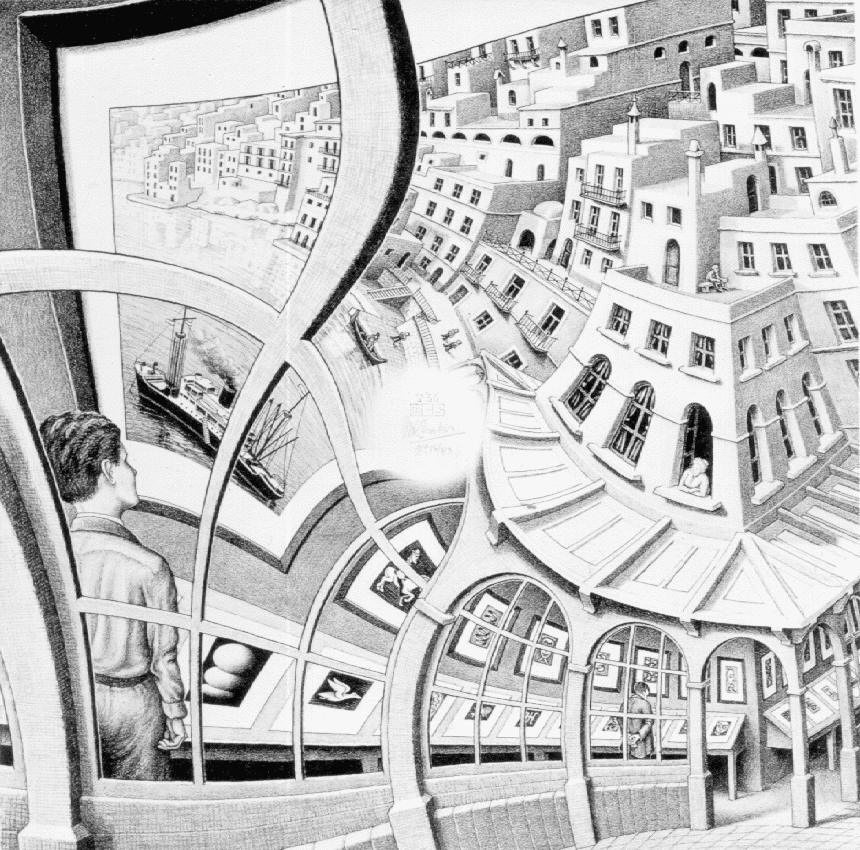
\includegraphics[width=0.5\columnwidth]{GalleriaStampe} 
%\caption[An example of a floating figure]{An example of a floating figure (a reproduction from the \emph{Gallery of prints}, M.~Escher,\index{Escher, M.~C.} from \url{http://www.mcescher.com/}).} % The text in the square bracket is the caption for the list of figures while the text in the curly brackets is the figure caption
%\label{fig:gallery} 
%\end{figure}

%\lipsum[10] % Dummy text

%------------------------------------------------

\subsection{Subsection}

\lipsum[11] % Dummy text

\subsubsection{Subsubsection}

\lipsum[12] % Dummy text

\begin{description}
\item[Word] Definition
\item[Concept] Explanation
\item[Idea] Text
\end{description}

\lipsum[12] % Dummy text

\begin{itemize}[noitemsep] % [noitemsep] removes whitespace between the items for a compact look
\item First item in a list
\item Second item in a list
\item Third item in a list
\end{itemize}

\subsubsection{Table}



\begin{table}[hbt]
\caption{Table of Grades}
\centering
\begin{tabular}{llr}
\toprule
\multicolumn{2}{c}{Name} \\
\cmidrule(r){1-2}
First name & Last Name & Grade \\
\midrule
John & Doe & $7.5$ \\
Richard & Miles & $2$ \\
\bottomrule
\end{tabular}
\label{tab:label}
\end{table}

Reference to Table~\vref{tab:label}. % The \vref command specifies the location of the reference

%------------------------------------------------

\subsection{Figure Composed of Subfigures}

Reference the figure composed of multiple subfigures as Figure~\vref{fig:esempio}. Reference one of the subfigures as Figure~\vref{fig:ipsum}. % The \vref command specifies the location of the reference


%----------------------------------------------------------------------------------------
%	BIBLIOGRAPHY
%----------------------------------------------------------------------------------------

\renewcommand{\refname}{\spacedlowsmallcaps{References}} % For modifying the bibliography heading

\bibliographystyle{unsrt}

\bibliography{sample.bib} % The file containing the bibliography











%----------------------------------------------------------------------------------------

\end{document}